% Created 2017-11-17 Fri 12:48
% Intended LaTeX compiler: pdflatex
\documentclass[11pt]{article}
\usepackage[utf8]{inputenc}
\usepackage[T1]{fontenc}
\usepackage{graphicx}
\usepackage{grffile}
\usepackage{longtable}
\usepackage{wrapfig}
\usepackage{rotating}
\usepackage[normalem]{ulem}
\usepackage{amsmath}
\usepackage{textcomp}
\usepackage{amssymb}
\usepackage{capt-of}
\usepackage{hyperref}
\usepackage{amsmath}
\author{Jake Brawer}
\date{\today}
\title{Assignment 8}
\hypersetup{
 pdfauthor={Jake Brawer},
 pdftitle={Assignment 8},
 pdfkeywords={},
 pdfsubject={},
 pdfcreator={Emacs 25.3.1 (Org mode 9.1.2)}, 
 pdflang={English}}
\begin{document}

\maketitle

\section*{Problem 1}
\label{sec:orgdb731c4}
\subsection*{a)}
\label{sec:org10c2986}
\begin{verbatim}
d <- read.csv("http://www.stat.yale.edu/~jtc5/238/data/cost-of-the-muse.csv")

ages <- d$Age

novlsts <- ages[d$Type == "Novels"]
pts <- ages[d$Type == "Poems"]
nfcts <- ages[d$Type == "Nonfiction"]

par(mfrow = c(3,1))
rg <- range(ages)

hist(novlsts, 100, xlim = rg, col="red")
hist(pts, 100, xlim = rg, col="blue")
hist(nfcts, 100, xlim = rg, col="green")
\end{verbatim}

\begin{center}
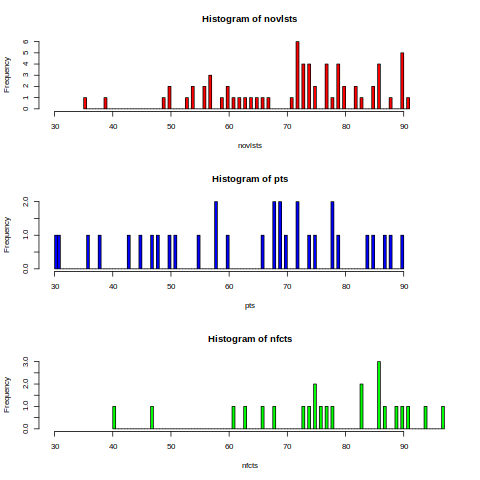
\includegraphics[width=.9\linewidth]{hist.png}
\end{center}

\subsection*{b)}
\label{sec:orgb7a4077}

\begin{verbatim}
lik <- function(th){
  mu1 <- th[1]; mu2 <- th[2]; mu3 <- th[3]
  s1 <- th[4]; s2 <- th[5]; s3 <- th[6]
  return(
    prod(dnorm(novlsts, mean=mu1, sd = s1)) *
    prod(dnorm(pts, mean=mu2, sd = s2)) *
    prod(dnorm(nfcts, mean=mu3, sd = s3))
  )
}
prior <- function(th){
  mu1 <- th[1]; mu2 <- th[2]; mu3 <- th[3]
  s1 <- th[4]; s2 <- th[5]; s3 <- th[6]
  return(prod(dunif(th, 0, 100)))
}

post <- function(th){
  s1 <- th[4]; s2 <- th[5]; s3 <- th[6]
  if((s1 < 0) | (s2 < 0) | (s3 < 0))return(0)
  return(prior(th) * lik(th))
}



MCMC <- function(reps, th){
  path <- matrix(0, nrow=reps, ncol=6)
  path[1, ] <- th
  for(i in 2:reps)
  {
    candidate <- th + rnorm(6)
    ratio <- post(candidate)/post(th)

    if(runif(1) < ratio) th <- candidate

    path[i, ] <- th
  }
  return(path)
}

reps <- 10000
strt <- c(65, 65, 65, 20, 20 , 20)

results <- MCMC(10000, strt)
mu1 <-  results[, 1]
mu2 <-  results[, 2]
mu3 <-  results[, 3]
sd1 <-  results[, 4]
sd2 <-  results[, 5]
sd3 <-  results[, 6]


qts <- c(0.025, 0.5, 0.975)

\end{verbatim}

\begin{center}
\begin{tabular}{r}
0.025\\
0.5\\
0.975\\
\end{tabular}
\end{center}



Novelist \(\mu\) credible intervals (0.025, 0.5, 0.97, respectively)
\begin{verbatim}
quantile(mu1, qts)
\end{verbatim}

\begin{center}
\begin{tabular}{r}
68.279693490428\\
71.4616761425772\\
74.8208908432986\\
\end{tabular}
\end{center}

Novelist \(SD\) credible intervals (0.025, 0.5, 0.97, respectively)
\begin{verbatim}
quantile(sd1, qts)
\end{verbatim}

\begin{center}
\begin{tabular}{r}
11.3638852594947\\
13.2705816035933\\
15.8373466476875\\
\end{tabular}
\end{center}

Poets \(\mu\) credible intervals (0.025, 0.5, 0.97, respectively)
\begin{verbatim}
quantile(mu2, qts)
\end{verbatim}

\begin{center}
\begin{tabular}{r}
57.1944221434365\\
63.2242358562457\\
69.0383701320644\\
\end{tabular}
\end{center}

Novelist \(SD\) credible intervals (0.025, 0.5, 0.97, respectively)
\begin{verbatim}
quantile(sd2, qts)
\end{verbatim}

\begin{center}
\begin{tabular}{r}
14.025471795276\\
17.9889332578746\\
24.1268678417386\\
\end{tabular}
\end{center}

Nonfiction writers \(\mu\) credible intervals (0.025, 0.5, 0.97, respectively)
\begin{verbatim}
quantile(mu3, qts)
\end{verbatim}

\begin{center}
\begin{tabular}{r}
70.8826163141118\\
76.6621468998993\\
82.2454072795531\\
\end{tabular}
\end{center}

Nonfiction writers \(SD\) credible intervals (0.025, 0.5, 0.97, respectively)
\begin{verbatim}
quantile(sd3, qts)
\end{verbatim}

\begin{center}
\begin{tabular}{r}
11.2462241539382\\
14.8611998181229\\
20.5064952415497\\
\end{tabular}
\end{center}

\subsection*{c)}
\label{sec:org06583a8}

\begin{verbatim}
df <- (as.data.frame(results))
names(df) <- c("mu1", "mu2", "mu3", "sd1", "sd2", "sd3")

# novelist - poets
delta1 <- df$mu1 - df$mu2
# nonfiction writers - poets
delta2 <- df$mu3 - df$mu2

\end{verbatim}


\begin{verbatim}
par(mfrow = c(2,1))

hist(delta1)
hist(delta2)
\end{verbatim}

\begin{center}
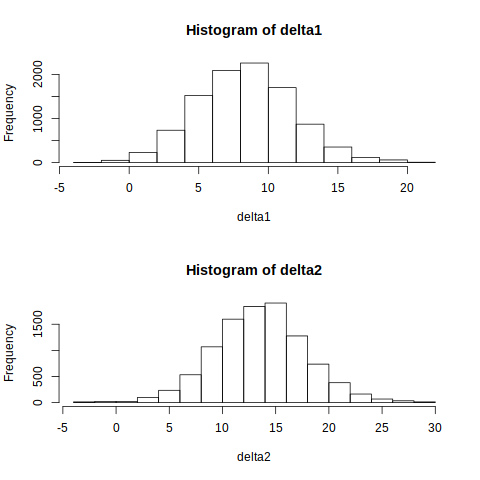
\includegraphics[width=.9\linewidth]{hist2.png}
\end{center}


Novelist - poets credible intervals (0.025, 0.975)
\begin{verbatim}
quantile(delta1, c(0.025,0.975))
\end{verbatim}

\begin{center}
\begin{tabular}{r}
1.82649328592878\\
15.4865634533126\\
\end{tabular}
\end{center}


Nonfiction writers - poets credible intervals (0.025, 0.975)
\begin{verbatim}
quantile(delta2, c(0.025,0.975))
\end{verbatim}

\begin{center}
\begin{tabular}{r}
5.03124181787953\\
22.2888167376865\\
\end{tabular}
\end{center}

\subsection*{d)}
\label{sec:org464e5e3}

\begin{verbatim}
delta3 <-  delta2 - delta1
mean(delta3 > 0)
\end{verbatim}

\begin{verbatim}
0.9403
\end{verbatim}

\section*{Problem 2}
\label{sec:orge425af5}
\begin{verbatim}
library('rjags')
mymodel <- "
  model {
    for(i in 1:length(novlsts)){
      novlsts[i] ~ dnorm(mu1 , tau1)
    }
    for(i in 1:length(pts)){
      pts[i] ~ dnorm(mu2 , tau2)
    }
    for(i in 1:length(nfcts)){
      nfcts[i] ~ dnorm(mu3 , tau3)
    }
  mu1 ~ dunif(0, 100)
  mu2 ~ dunif(0, 100)
  mu3 ~ dunif(0, 100)
  sig1 ~ dunif(0, 100)
  sig2 ~ dunif(0, 100)
  sig3 ~ dunif(0, 100)
  tau1 <- 1/(sig1 ^2)
  tau2 <- 1/(sig2 ^2)
  tau3 <- 1/(sig3 ^2)
}
"
jm <- jags.model (file = textConnection ( mymodel ),
                  data=list(novlsts=novlsts ,
                            pts=pts,
                            nfcts=nfcts),
                  inits=list(mu1 =65, sig1 =20,
                             mu2 =65, sig2 =20,
                             mu3 =65, sig3 =20))
cs <- coda.samples (jm , c('mu1','sig1','mu2','sig2', 'mu3', 'sig3'), 100000)
s <- as.data.frame (cs [[1]])
\end{verbatim}

\begin{verbatim}
qts <- c(0.025, 0.5, 0.975)
quantile(s$mu1, qts)
\end{verbatim}

\begin{center}
\begin{tabular}{rr}
0.025 & 68.2467778031878\\
0.5 & 71.4358081522129\\
0.975 & 74.6465196684498\\
\end{tabular}
\end{center}


\begin{verbatim}
qts <- c(0.025, 0.5, 0.975)
quantile(s$sig1, qts)
\end{verbatim}

\begin{center}
\begin{tabular}{rr}
0.025 & 11.2466288801889\\
0.5 & 13.2170804017298\\
0.975 & 15.8769467329275\\
\end{tabular}
\end{center}

\begin{verbatim}
qts <- c(0.025, 0.5, 0.975)
quantile(s$mu2, qts)
\end{verbatim}

\begin{center}
\begin{tabular}{rr}
0.025 & 56.8408695246123\\
0.5 & 63.1785840942802\\
0.975 & 69.5388634163273\\
\end{tabular}
\end{center}

\begin{verbatim}
qts <- c(0.025, 0.5, 0.975)
quantile(s$sig2, qts)
\end{verbatim}

\begin{center}
\begin{tabular}{rr}
0.025 & 14.032656853907\\
0.5 & 17.7715410431306\\
0.975 & 23.4585322202547\\
\end{tabular}
\end{center}

\begin{verbatim}
qts <- c(0.025, 0.5, 0.975)
quantile(s$mu3, qts)
\end{verbatim}

\begin{center}
\begin{tabular}{rr}
0.025 & 70.8154910038315\\
0.5 & 76.8770028433609\\
0.975 & 82.9686162380408\\
\end{tabular}
\end{center}

\begin{verbatim}
qts <- c(0.025, 0.5, 0.975)
quantile(s$sig3, qts)
\end{verbatim}

\begin{center}
\begin{tabular}{rr}
0.025 & 11.1451597067461\\
0.5 & 14.6521626614445\\
0.975 & 20.4100336403886\\
\end{tabular}
\end{center}

\begin{verbatim}
dt1 <- s$mu1 - s$mu2
dt2 <- s$mu3 - s$mu2

par(mfrow = c(2,1))

hist(dt1)
hist(dt2)
\end{verbatim}

\begin{center}
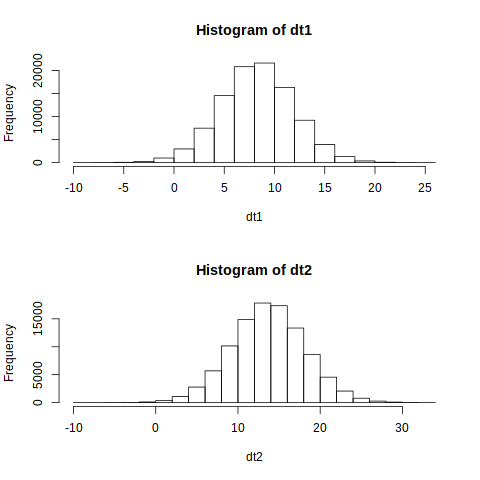
\includegraphics[width=.9\linewidth]{fig4.png}
\end{center}

\begin{verbatim}
dt3 <- dt2 - dt1
mean(dt3 > 0)
\end{verbatim}

\begin{verbatim}
0.93957
\end{verbatim}

\section*{Problem 3}
\label{sec:org119b9d3}
\subsection*{a)}
\label{sec:org0265e16}
\begin{verbatim}
xTrt <- 56
  xCtrl <- 84
  modelHeart <- "
    model{
      xTrt ~ dbin(pTrt, 2051)
      xCtrl ~ dbin(pCtrl, 2030)

      pTrt ~ dunif(0, 1)
      pCtrl ~ dunif(0, 1)
    }
  "

  jm <- jags.model (file = textConnection ( modelHeart ),
                    data=list(xTrt=xTrt, xCtrl=xCtrl),
                    )
  cs <- coda.samples (jm , c("pTrt", "pCtrl"), 100000)
  s <- as.data.frame (cs [[1]])


  par(mfrow = c(2,1))
  hist(s$pCtrl)
  hist(s$pTrt)
\end{verbatim}

\begin{center}
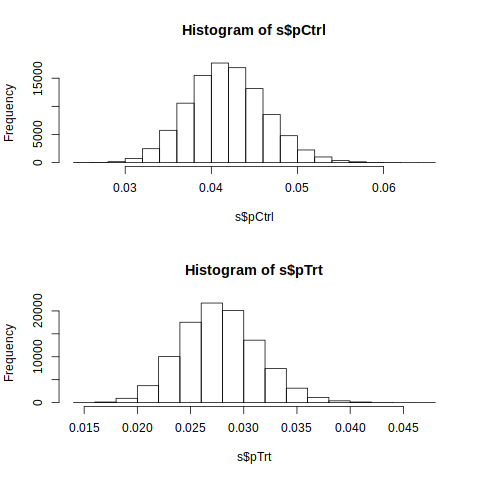
\includegraphics[width=.9\linewidth]{fig1.png}
\end{center}

\subsection*{b)}
\label{sec:org23a6fae}

\begin{verbatim}
qt <- c(0.025, 0.975 )
quantile(s$pCtrl, qt)
\end{verbatim}

\begin{center}
\begin{tabular}{rr}
0.025 & 0.0335144495945179\\
0.975 & 0.0508070951553886\\
\end{tabular}
\end{center}

\begin{verbatim}
quantile(s$pTrt, qt)
\end{verbatim}

\begin{center}
\begin{tabular}{rr}
0.025 & 0.0211767269637845\\
0.975 & 0.0353057663606585\\
\end{tabular}
\end{center}

\subsection*{c)}
\label{sec:orgd2107d4}

\begin{verbatim}
quantile( 100 * (s$pCtrl - s$pTrt)/s$pCtrl, qt)
\end{verbatim}


\begin{center}
\begin{tabular}{rr}
0.025 & 7.90152955146893\\
0.975 & 52.4127972295888\\
\end{tabular}
\end{center}

\section*{4)}
\label{sec:org5e2d779}

\subsection*{a)}
\label{sec:orgfdc7a89}
$P(\theta_{trt}) = P(\theta_{ctrl}) = U(0,1) = Beta(1,1)$\\
$L(\theta_{trt}) = Beta(56, 1995), L(\theta_{ctrl}) = Beta(84, 1946)$\\
Thus the post. dist. for $\theta_{trt}$ is: $B(56 + 1, 1995 + 1)$ and the post
dist for $\theta_{ctrl}$ is: $Beta(84 + 1, 1946 + 1)$

\subsection*{b)}
\label{sec:org4b1616f}

Credible intervals for \(\theta_{\text{trt}}\)
\begin{verbatim}
i1 <- qbeta(.025, 57, 1996)
i2 <- qbeta(.975, 57, 1996)

sprintf("The credible interval is [%s, %s]", i1, i2)
\end{verbatim}

\begin{verbatim}
The credible interval is [0.021105000440969, 0.0352939682359724]
\end{verbatim}


Credible intervals for \(\theta_{\text{ctrl}}\)
\begin{verbatim}
i1 <- qbeta(.025, 85, 1947)
i2 <- qbeta(.975, 85, 1947)

sprintf("The credible interval is [%s, %s]", i1, i2)
\end{verbatim}

\begin{verbatim}
The credible interval is [0.0335636928570328, 0.0509513571991438]
\end{verbatim}

\subsection*{c)}
\label{sec:org25d6481}

\begin{verbatim}
sTrt <- rbeta(10000, 57, 1996)
sCtrl <-  rbeta(10000, 85, 1947)

reduc <- (100* ( sCtrl - sTrt))/sCtrl
quantile(reduc, c(0.025, 0.975))
\end{verbatim}

\begin{center}
\begin{tabular}{r}
8.61584056106628\\
52.7245199349204\\
\end{tabular}
\end{center}
\end{document}